%=========================================================
% Mathematics Report Template - HD Standard
%=========================================================
\documentclass[11pt,a4paper]{article}

%---------------- Packages ----------------
\usepackage[utf8]{inputenc}
\usepackage[T1]{fontenc}
\usepackage{lmodern}
\usepackage{geometry}
\usepackage{multicol}
\geometry{a4paper, margin=2.5cm}
\usepackage{tikz}
\usetikzlibrary{calc}
\usetikzlibrary{angles,quotes} % for angle marks
\usepackage{tabularx}
\usepackage{booktabs}
\usetikzlibrary{arrows.meta, positioning}
\usepackage{float}
\usepackage{setspace}
\usepackage[skip=0.6\baselineskip, indent=0pt]{parskip} % no paragraph indent, vertical gap instead
\usepackage{algorithm}
\usepackage{algpseudocode}
% optional: make comments right-aligned with a pointer
\algrenewcommand\algorithmiccomment[1]{\hfill$\triangleright$~#1}

\usepackage{amsmath, amssymb, amsthm, mathtools} % math environments
\usepackage{mathrsfs}
\usepackage{bm}             % bold math symbols
\usepackage{physics}        % derivatives, bra-ket, etc.
\usepackage{enumitem}       % custom lists
\usepackage{tikz}           % diagrams
\usepackage{pgfplots}       % plots
\pgfplotsset{compat=1.18}
\usepackage{graphicx}       % figures
\usepackage{subcaption}     % subfigures
\usepackage{xcolor}         % colors
\usepackage{hyperref}       % hyperlinks
\hypersetup{colorlinks=true, linkcolor=black, citecolor=blue, urlcolor=blue}

%---------------- Theorem Environments ----------------
\newtheorem{theorem}{Theorem}[section]
\newtheorem{lemma}[theorem]{Lemma}
\newtheorem{proposition}[theorem]{Proposition}
\newtheorem{corollary}[theorem]{Corollary}
\theoremstyle{definition}
\newtheorem{definition}[theorem]{Definition}
\newtheorem{example}[theorem]{Example}
\theoremstyle{remark}
\newtheorem{remark}[theorem]{Remark}

%---------------- Title Page ----------------
\title{\textbf{Mini Project \\ Sydney Housing Price Prediction and Decision Support System}\\[6pt]
       \large {SIT307 -- Machine Learning}}
\author{Student Name: Bao Minh Tran \\
 Student ID: s224236373 \\
  Deakin University}
\date{August $26^{th}$, 2026}

%=========================================================
\begin{document}

%=========================================================
% Cover Page
%=========================================================
\begin{titlepage}
    \centering
    {\scshape\LARGE Deakin University}\\[0.2cm]
    {\large Faculty of Science, Engineering and Built Environment}\\[0.2cm]
    {\large School of IT}\\[1cm]
    
\includegraphics[width=6cm]{./figures/logo.jpg}\\[2cm]

    % Report title
    % {\Large \textbf{Technical Report}}\\[0.5cm]
    % {\huge \textbf{Towards Video Understanding: Action Recognition by PyTorchVideo}}\\[3cm]
    {\huge
    \setlength{\baselineskip}{1.2\baselineskip}
    \textbf{Sydney Housing Price Prediction and Decision Support System}
    \par
    }

    \vspace{2cm}

    {\Large \textbf{SIT307 – Machine Learning}}\\[0.5cm]
    {\Large Lecturer: A/Prof. Kewen Liao}\\[2cm]

    % Author info
    {\large Student Name: Bao Minh Tran}\\[0.5cm]
    {\large Student ID: s224236373}\\[0.5cm]
    {\large Email: s224236373@deakin.edu.au}\\[2cm]

    % Supervisor or Lecturer

    % Date
    {\large August $26^{th}$, 2026}

    \vfill
\end{titlepage}

\begin{abstract}
    \noindent
    This project establishes a full pipeline, including data scraping, wrangling, modelling, and insights delivery.
    Predicts residential sale price from observable listing characteristics for three contrasting Sydney suburbs (Blacktown, Chatswood, Mosman), and serves the trained model through a small web–based application using \texttt{streamlit}.
    The implementation of this project can be found in this GitHub repo \href{https://github.com/Trminh06-work/Sydney_housing.git}{Sydney\_housing}.
\end{abstract}

\setcounter{tocdepth}{2}
\tableofcontents
\newpage

%=========================================================
\section{Problem Definition and Data Collection}
\subsection{Problem definition and suburb selection}

An agency needs a tool estimating sale price from observable characteristics:
supervised regression, predicting $y \in \mathbb{R}^{+}$ from features $\mathbf{x}$.
The framing is hedonic \cite{rosen1974hedonic,malpezzi2003hedonic}. Accuracy alone is
insufficient, because the agency also needs to know when to distrust a prediction,
which motivates Section~4.

Three suburbs were chosen to span deliberately different markets, so location would be
a first-order predictor. They differ in level, spread and stock (Table~\ref{tab:suburbs}), i.e. Blacktown house-dominant and affordable, Chatswood
unit-dominant, Mosman mixed and premium. Suburb and type are entangled by construction,
so both are retained as inputs.

\begin{table}[H]
\centering\small
\begin{tabularx}{\textwidth}{@{}l XXX@{}}
\toprule
 & \textbf{Blacktown} & \textbf{Chatswood} & \textbf{Mosman} \\
\midrule
Retained sales $n$   & 79 & 62 & 47 \\
Median price         & \$950{,}000 & \$1{,}417{,}500 & \$1{,}760{,}000 \\
Mean price           & \$901{,}570 & \$1{,}716{,}668 & \$2{,}737{,}883 \\
Std.\ deviation      & \$334{,}345 & \$970{,}869 & \$2{,}116{,}702 \\
Range                & \$0.41--1.88M & \$0.70--4.80M & \$0.70--8.70M \\
Houses / Apartments  & 47 / 25 & 13 / 48 & 11 / 28 \\
Other stock          & 6 Twn, 1 Vil & 1 Twn & 4 Twn, 2 Ret, 2 Semi \\
\bottomrule
\end{tabularx}
\caption{Suburb contrast, computed in the notebook from the retained sample
($n=188$). Twn = townhouse, Ret = retirement living, Semi = semi-detached.}
\label{tab:suburbs}
\end{table}

\subsection{Collection, quality and limitations}

Records came from public \texttt{domain.com.au} sold listings \cite{domain2026sold},
with context from Domain profiles \cite{domain2026suburb} and ABS SEIFA
\cite{abs2021seifa}. realestate.com.au was excluded, as it denied programmatic access and
REA Group has an enforcement record \cite{om2024rea}. Every row carries
\texttt{source\_url} and \texttt{retrieved\_at} for verification purpose.

The original collection comprises of 239 properties, with missing values present in different columns.
Therefore, we aggressively discard incomplete rows, such that, there are more than 100 properties left with at least 30 properties in each suburb left.
Having removed the incomplete rows, \texttt{area\_sqm} is the only single source of missingness, so it
alone was exempted. Its remaining 64 gaps (34\%) are imputed inside the modelling pipeline.
Fortunately, three of those six columns are not model inputs, and it cost 27 Mosman sales, contributing to the sparse Mosman tail in the price distribution. Cross-validating
all three models on both the full and filtered sets confirms it is nonetheless the better choice, rather than keeping the missing values and conduct imputation in the modelling pipeline.

Noticeably, there are three apparent limitations. First, sales span only March--August 2026 with uneven coverage, so
the temporal term cannot be extrapolated. Second, \texttt{area\_sqm} remains $34\%$ missing, so that column depends on imputation.
Third, the SEIFA and \texttt{suburb\_*} columns resolve to three distinct rows, restating the suburb label rather than adding property-level information.

We also identify a potential source of bias is selection on price disclosure. Collection filtered to
listings showing a price, so withheld-price sales are absent by construction, and withholding is not random. The sample therefore under-represents the top of each distribution, most acutely in Mosman.
Recovering those sales requires the NSW Valuer General's statutory register \cite{vgnsw2026psi}, which records every transfer regardless of advertised disclosure.

%=========================================================



%=========================================================
\newpage
\section{Data Understanding and Feature Engineering}
\subsection{Distribution, suburbs and time}

Prices are heavily right-skewed, yet near-symmetric on a log axis
(Figure~\ref{fig:dist}). This implies the price effects are
multiplicative, and thus, the price target is logarithmically scaled in the modelling pipeline. Dispersion grows with
level, Mosman's standard deviation (\$2.12M) is over six times Blacktown's (\$334k); however,
extreme values are a property of the market, not outliers.

\begin{figure}[H]
\centering
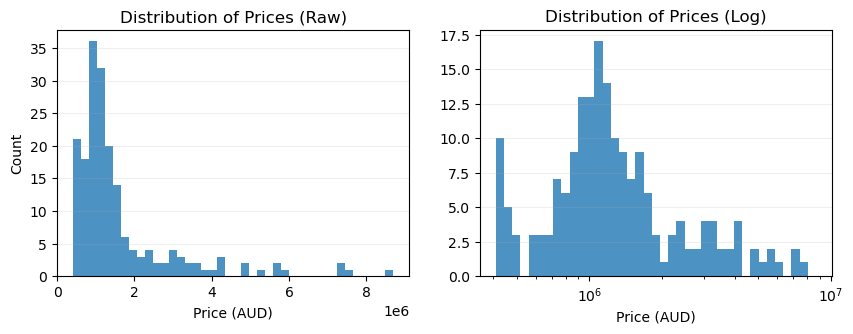
\includegraphics[width=0.86\textwidth]{figures/p2_price_dist.png}\\[1.4ex]
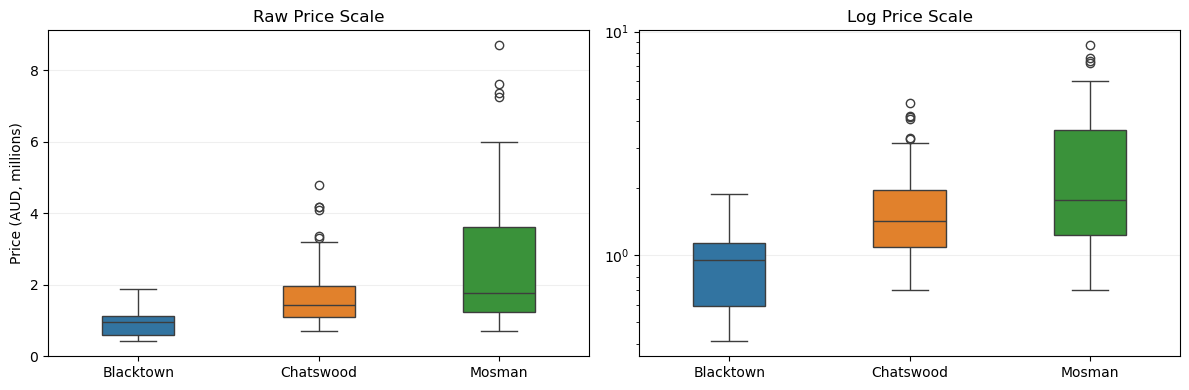
\includegraphics[width=0.86\textwidth]{figures/p2_suburb_box.png}
\caption{Price distribution in raw and log scale (top); by suburb, raw and log scale (bottom).}
\label{fig:dist}
\end{figure}

The temporal view is least trustworthy, across six months, badly unbalanced monthly coverage,
and no repeated seasonal cycle (Figure~\ref{fig:trend}). The correlation heatmap
(Figure~\ref{fig:corr}) shows the SEIFA block is redundant with suburb.

\begin{figure}[H]
\centering
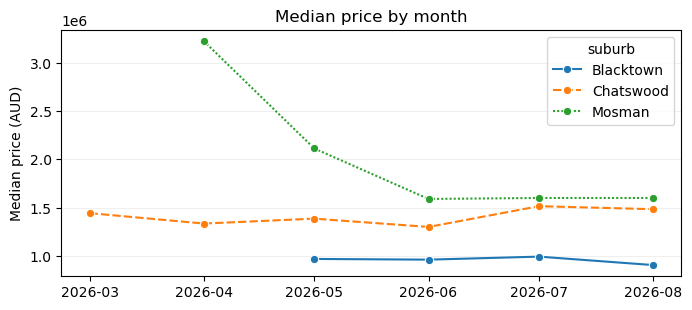
\includegraphics[width=0.72\textwidth]{figures/p2_time_trend.png}
\caption{Median price by month. Coverage is uneven: Blacktown contributes no sales
before May, Chatswood only two in August.}
\label{fig:trend}
\end{figure}

\begin{figure}[H]
\centering
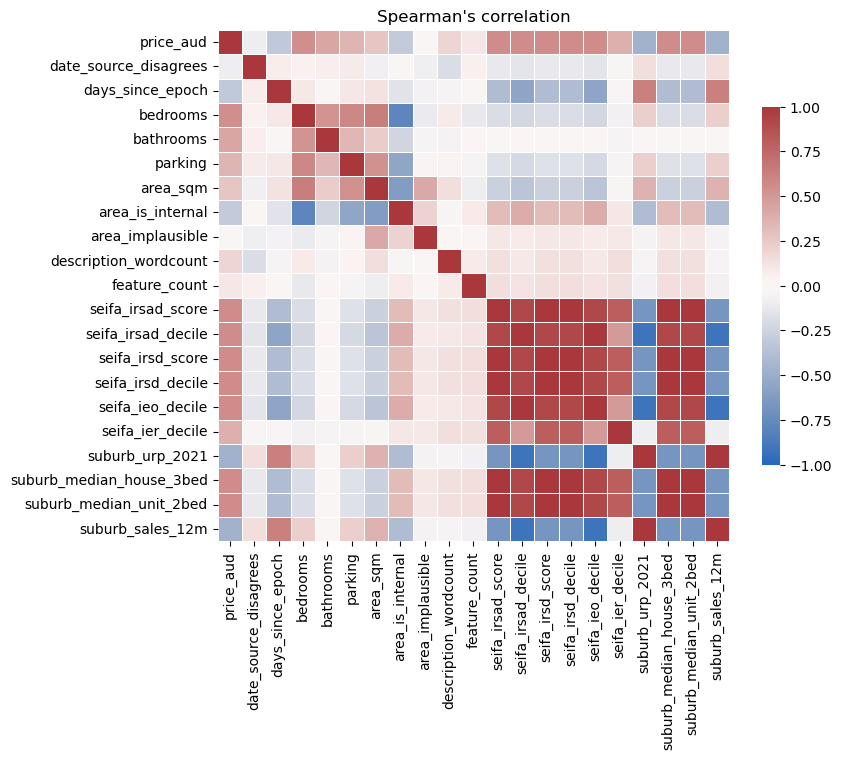
\includegraphics[width=0.55\textwidth]{figures/p2_corr_heatmap.png}
\caption{Spearman $\rho$ correlation, target included. The ten SEIFA and
\texttt{suburb\_*} columns take only three distinct rows, one per suburb, and are
mutually correlated at $\approx 1$.}
\label{fig:corr}
\end{figure}

\begin{figure}[H]
\centering
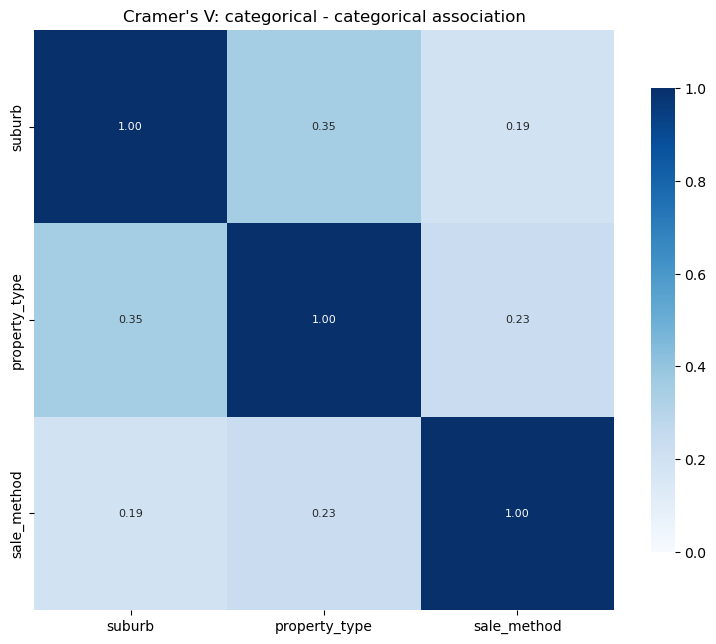
\includegraphics[width=0.35\textwidth]{figures/p2_cramer.png}
\caption{Cramer's $V$ correlation, target excluded}
\label{fig:cramer}
\end{figure}

\subsection{Expected drivers and engineered features}

Three variables were nominated beforehand as most influential, i.e. \textbf{suburb}
(location dominated every comparison above), \textbf{property\_type} (houses and units
priced by different logic) and \textbf{price tercile} (to expose whether accuracy
depends on position in the price range). From these, \texttt{is\_unit} collapses six
types into a land-versus-strata binary, avoiding near-empty categories such as Villa
($n=1$); \texttt{bed\_bath} and \texttt{beds\_x\_unit} summarise size and let a
bedroom's value differ by type, \texttt{t} and \texttt{month} carry time, six
\texttt{kw\_*} flags recover condition signals from agent text.

Remarkably, only two of three survive as inputs, since the price tercile is derived from the target, which leaks a lot of information to the model.
Thus, it serves diagnosis but is never available at prediction time, a limitation of the guess rather than the engineering.
The third nominated driver, size, is measured two ways, i.e. directly by \texttt{area\_sqm}, and indirectly by the room-count composites.
The feature set therefore encodes the intended understanding (location first, type second, size third), though the direct size (\texttt{area\_sqm}) measurement rests on imputation for a third of the sample.

%=========================================================


%=========================================================
\newpage
\section{Model Development and Evaluation}
\subsection{Models, pipeline and prior expectation}

Three models represent different inductive biases. \textbf{Ridge}, regularised linear:
with $n=188$ and one-hot categoricals the design matrix is wide, and the $L_2$ penalty
stabilises correlated inputs such as \texttt{bedrooms} and \texttt{bed\_bath}.
\textbf{Random Forest} bags deep trees, capturing interactions unprompted.
\textbf{AdaBoost} fits residuals sequentially, chasing structure the others miss but
most sensitive to atypical records.

All preprocessing sits inside the pipeline (median imputation, standardisation, and
one-hot encoding with \texttt{min\_frequency=3}), so it refits within every fold and
cannot leak, which is important for \texttt{area\_sqm}, whose 64 missing values are filled
from each training fold's median. The target is $\log(\text{price})$. Data is split 131/57 and tuned by grid
search under 5-fold cross-validation on RMSE.

\textbf{Prediction.} The ensembles were expected to win, since a small dataset mixing
categorical and numeric inputs across three different suburbs favours trees, more expressive power than Ridge.

\subsection{Results and recommendation}

\begin{table}[H]
\centering\small
\begin{tabularx}{\textwidth}{@{}l X r r r r r r@{}}
\toprule
\textbf{Model} & \textbf{Best parameters} & \textbf{RMSE} & \textbf{MAPE\%} & \textbf{MAE} & \textbf{$R^2_{cv}$} & \textbf{$R^2_{tr}$} & \textbf{gap} \\
\midrule
Ridge         & \texttt{alpha}=0.231                                & \textbf{0.2055} & \textbf{16.78} & \textbf{0.1652} & 0.9131 & 0.9358 & \textbf{0.0227} \\
Random Forest & \texttt{depth}=4, \texttt{leaf}=3, \texttt{n}=100    & 0.2170 & 16.97 & 0.1705 & 0.9030 & 0.9411 & 0.0380 \\
AdaBoost      & \texttt{lr}=0.05, \texttt{n}=300                     & 0.2257 & 18.15 & 0.1814 & 0.8951 & 0.9321 & 0.0370 \\
\bottomrule
\end{tabularx}
\caption{Out-of-fold results on the training split (RMSE, MAE and $R^2$ in log
units; MAPE back-transformed to AUD). All three share identical folds.}
\label{tab:models}
\end{table}

From the table, no model underfits (all achieve $R^2_{cv} \geq 0.89$). Indeed, they do not overfit badly, since all gap are insignificant, at most 0.038 in \texttt{Random Forest}.
Looking at the learning curves, it progressively falls when the fit size increases, which is indicative of allowing more traning samples may improve models' performance.

\begin{figure}[H]
\centering
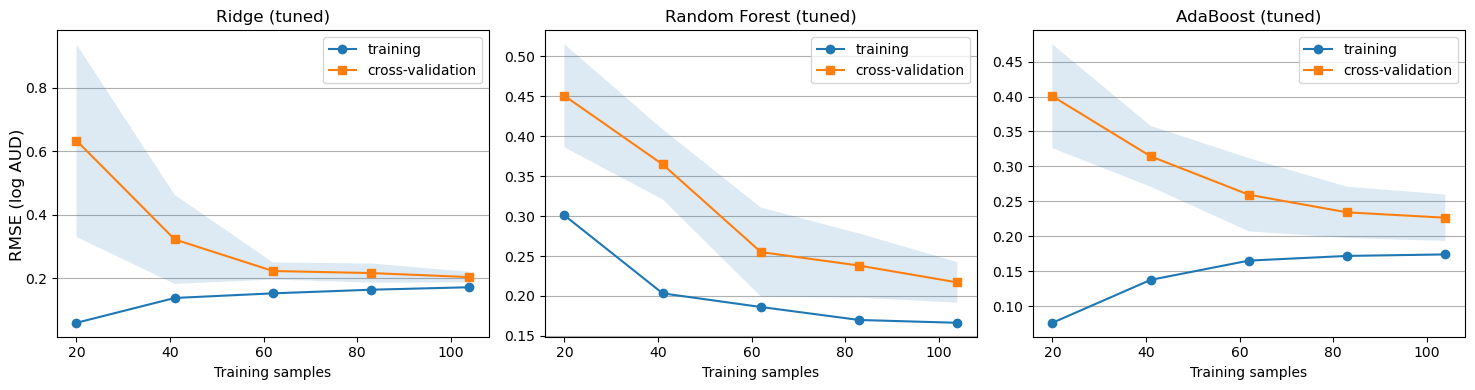
\includegraphics[width=\textwidth]{figures/p3_learning_curves.png}
\caption{Learning curves. The cross-validation curve is still falling at the largest
fit size (roughly 105 rows: four fifths of the 131 training rows) for all three models.}
\label{fig:lc}
\end{figure}

\begin{table}[H]
\centering\small
\begin{tabular}{@{}c c@{}}
\toprule
\textbf{Model} & \textbf{Corr}  \\
\midrule
\texttt{Ridge}    & 0.095  \\
\texttt{Random Forest} & 0.416  \\
\texttt{AdaBoost} & 0.330  \\
\bottomrule
\end{tabular}
\caption{Pearson $\tau$ correlation between models' absolute residual errors and price target.}
\label{tab:residuals_analysis}
\end{table}

Considering the table above, evidently, \texttt{Ridge} has errors that do not scale with price (correlation 0.095, against 0.416 and 0.330).
This is the most decisive quantitative result driving our choice of best model. Let us present how each model produce residual errors.

\begin{figure}[H]
\centering
\begin{subfigure}{\textwidth}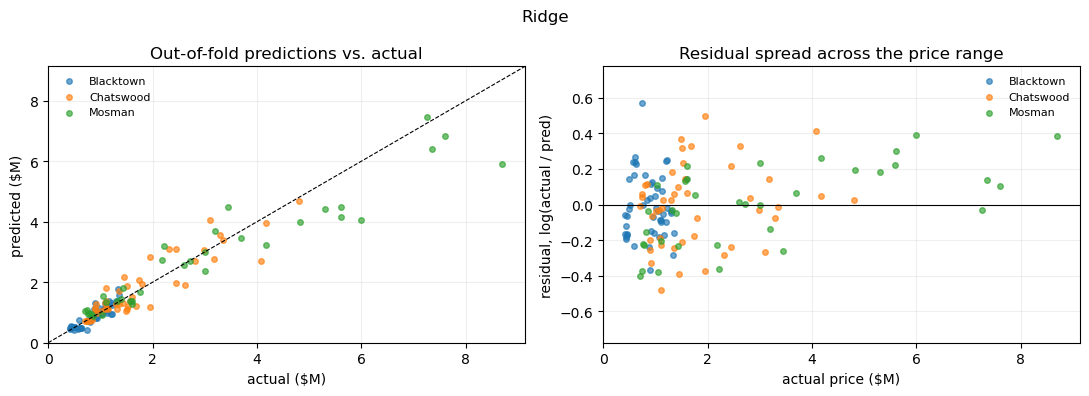
\includegraphics[width=\linewidth]{figures/p4_resid_ridge.png}\end{subfigure}
\begin{subfigure}{\textwidth}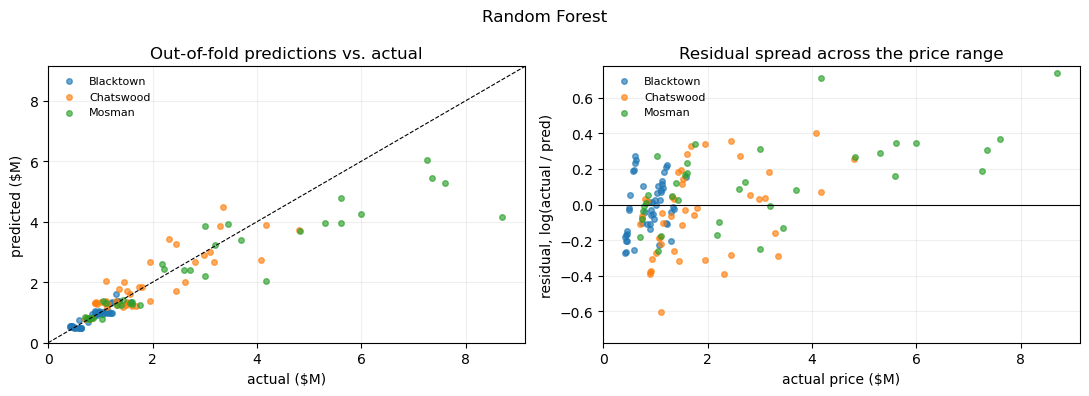
\includegraphics[width=\linewidth]{figures/p4_resid_rf.png}\end{subfigure}
\begin{subfigure}{\textwidth}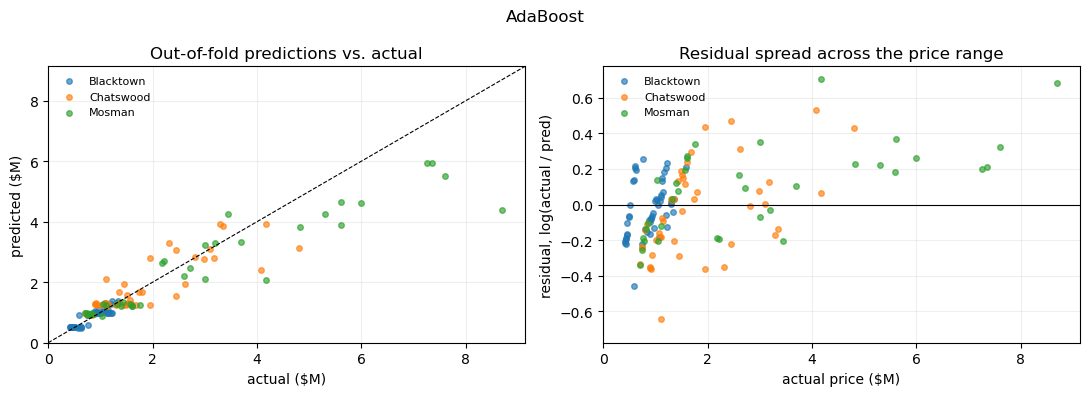
\includegraphics[width=\linewidth]{figures/p4_resid_ada.png}\end{subfigure}
\caption{Out-of-fold predictions and residual spread, coloured by suburb: Ridge
(top), Random Forest (middle) and AdaBoost (bottom).}
\label{fig:resid}
\end{figure}


\textbf{The prior expectation was not supported.} \texttt{Ridge} leads every cross-validated
metric, is least over-fitted, and is the only model whose accuracy holds across the
price range, which is more useful than one accurate only where data is dense. With
\texttt{area\_sqm} imputed for a third of rows, the usable signal is largely additive in
log-price, so the ensembles' flexibility bought variance at $n=188$. On the untouched test set, \texttt{Ridge}
scores RMSE 0.2199, MAPE 17.51\%, $R^2$ 0.8096, or roughly $\pm 25\%$. Being slightly
worse than the cross-validated 0.2055 is the expected direction, and small enough to
indicate tuning did not badly overfit the folds.

%=========================================================


%=========================================================
% \newpage
\section{Investigating Prediction Failures}
\subsection{The five largest errors}

Failures are ranked on $\log(\text{actual}/\text{predicted})$, not dollars:
$|\text{dollar error}|$ largely restates price, whereas the log residual is scale-free
and finds where the model is genuinely confused.

\begin{table}[H]
\centering\small
\begin{tabular}{@{}l l c c r r r@{}}
\toprule
\textbf{Suburb} & \textbf{Type} & \textbf{Bed} & \textbf{Bath} & \textbf{Actual} & \textbf{Predicted} & \textbf{Err (\%)} \\
\midrule
Mosman    & Apartment & 1 & 1 & \$1{,}570{,}000 & \$845{,}911     & $+46.1$ \\
Chatswood & Apartment & 3 & 3 & \$1{,}385{,}888 & \$2{,}365{,}823 & $-70.7$ \\
Chatswood & Apartment & 2 & 2 & \$2{,}150{,}000 & \$1{,}300{,}159 & $+39.5$ \\
Blacktown & House     & 3 & 2 & \$1{,}000{,}000 & \$1{,}516{,}701 & $-51.7$ \\
Chatswood & Apartment & 1 & 1 & \$1{,}030{,}000 & \$703{,}932     & $+31.7$ \\
\bottomrule
\end{tabular}
\caption{The five largest prediction errors on the held-out test set (Ridge).}
\label{tab:worst}
\end{table}

Four of five are apartments, three sharing room counts with far cheaper units elsewhere.
The worst case, a one-bedroom Mosman apartment at \$1.57M against \$846k predicted, is
the clearest. In particular, room counts barely separate a 1-bed/1-bath unit from any other, and
where \texttt{area\_sqm} is missing it is replaced by the sample median, so the outlook
justifying its price is invisible to the model.
Five isolated cases could be outliers; whether they are is settled by asking if the same
errors recur across a group.

\begin{table}[H]
\centering\small
\begin{tabular}{@{}l l r r r@{}}
\toprule
\textbf{Cut} & \textbf{Segment} & \textbf{$n$} & \textbf{Mean $|$err$|$ (\%)} & \textbf{Signed bias (\%)} \\
\midrule
Suburb        & Blacktown & 29 & 11.7 & $-4.9$ \\
              & Chatswood & 16 & 25.6 & $-6.2$ \\
              & Mosman    & 12 & 20.9 & $-0.5$ \\
\addlinespace
Property type & Apartment & 30 & 21.9 & $-4.3$ \\
              & House     & 21 & 12.9 & $-6.0$ \\
\addlinespace
Price tercile & Low       & 19 & 13.7 & $-10.8$ \\
              & Mid       & 19 & 17.2 & $-4.1$ \\
              & High      & 19 & 21.7 & $+1.9$ \\
\bottomrule
\end{tabular}
\caption{Test-set error by segment. Negative bias indicates over-prediction. Minor
property types (townhouse, villa and retirement living; 6 sales combined) are omitted.}
\label{tab:seg}
\end{table}

Chatswood averages 25.6\% against Blacktown's 11.7\% despite mid-range prices,
so this is not merely a tail problem. Apartments average 21.9\% against 12.9\% for
houses. Signed bias flips from $-10.8\%$ in the low tercile to $+1.9\%$ in the high. In conclusion, the
model over-prices cheap homes and under-prices dear ones, regressing toward the mean and
disadvantaging owners of unusual properties.

\subsection{Limitations and when to distrust an estimate}

Units are inherently harder to model \emph{with these features}. Houses separate
tolerably by room counts, whereas two apartments identical in bedrooms, bathrooms and
parking can differ several-fold on floor level, aspect and outlook, none of which is
recorded here. What would most improve performance is missing measurement, not a better
algorithm.

Remarkably, estimates for one-bedroom units are least reliable, estimates at
either price extreme are biased toward the middle, and any estimate outside
March--August 2026 extrapolates the temporal term with no evidence.

%=========================================================


%=========================================================
% \newpage
\section{Final Deployment and Reflection}
\subsection{The application}

The deployed model is the Ridge pipeline refit on all 188 sales. The split existed to
obtain an unbiased error estimate, and once that is recorded there is no reason to
discard 30\% of the evidence. It is serialised to \texttt{src/model.joblib} with its column lists, so
the app builds feature rows from the definitions used in training.

\texttt{src/app.py} is a Streamlit prototype loading that bundle, offering a
single-property form and a CSV upload. Inputs are only fields readable off a listing,
including floor or land area, which can be left blank. Derived terms are
computed internally. The app exponentiates before display and reports
a $\pm 20\%$ band rather than a point estimate.

\begin{verbatim}
pip install -r requirements.txt
jupyter nbconvert --to notebook --execute --inplace notebooks/lab.ipynb
streamlit run src/app.py        # from the project root; serves localhost:8501
\end{verbatim}

The notebook must run first, since it writes \texttt{src/model.joblib}. Full instructions,
including rebuilding the dataset from the cached raw pages, are in \texttt{README.md}.

\begin{figure}[H]
\centering
\begin{subfigure}{0.49\textwidth}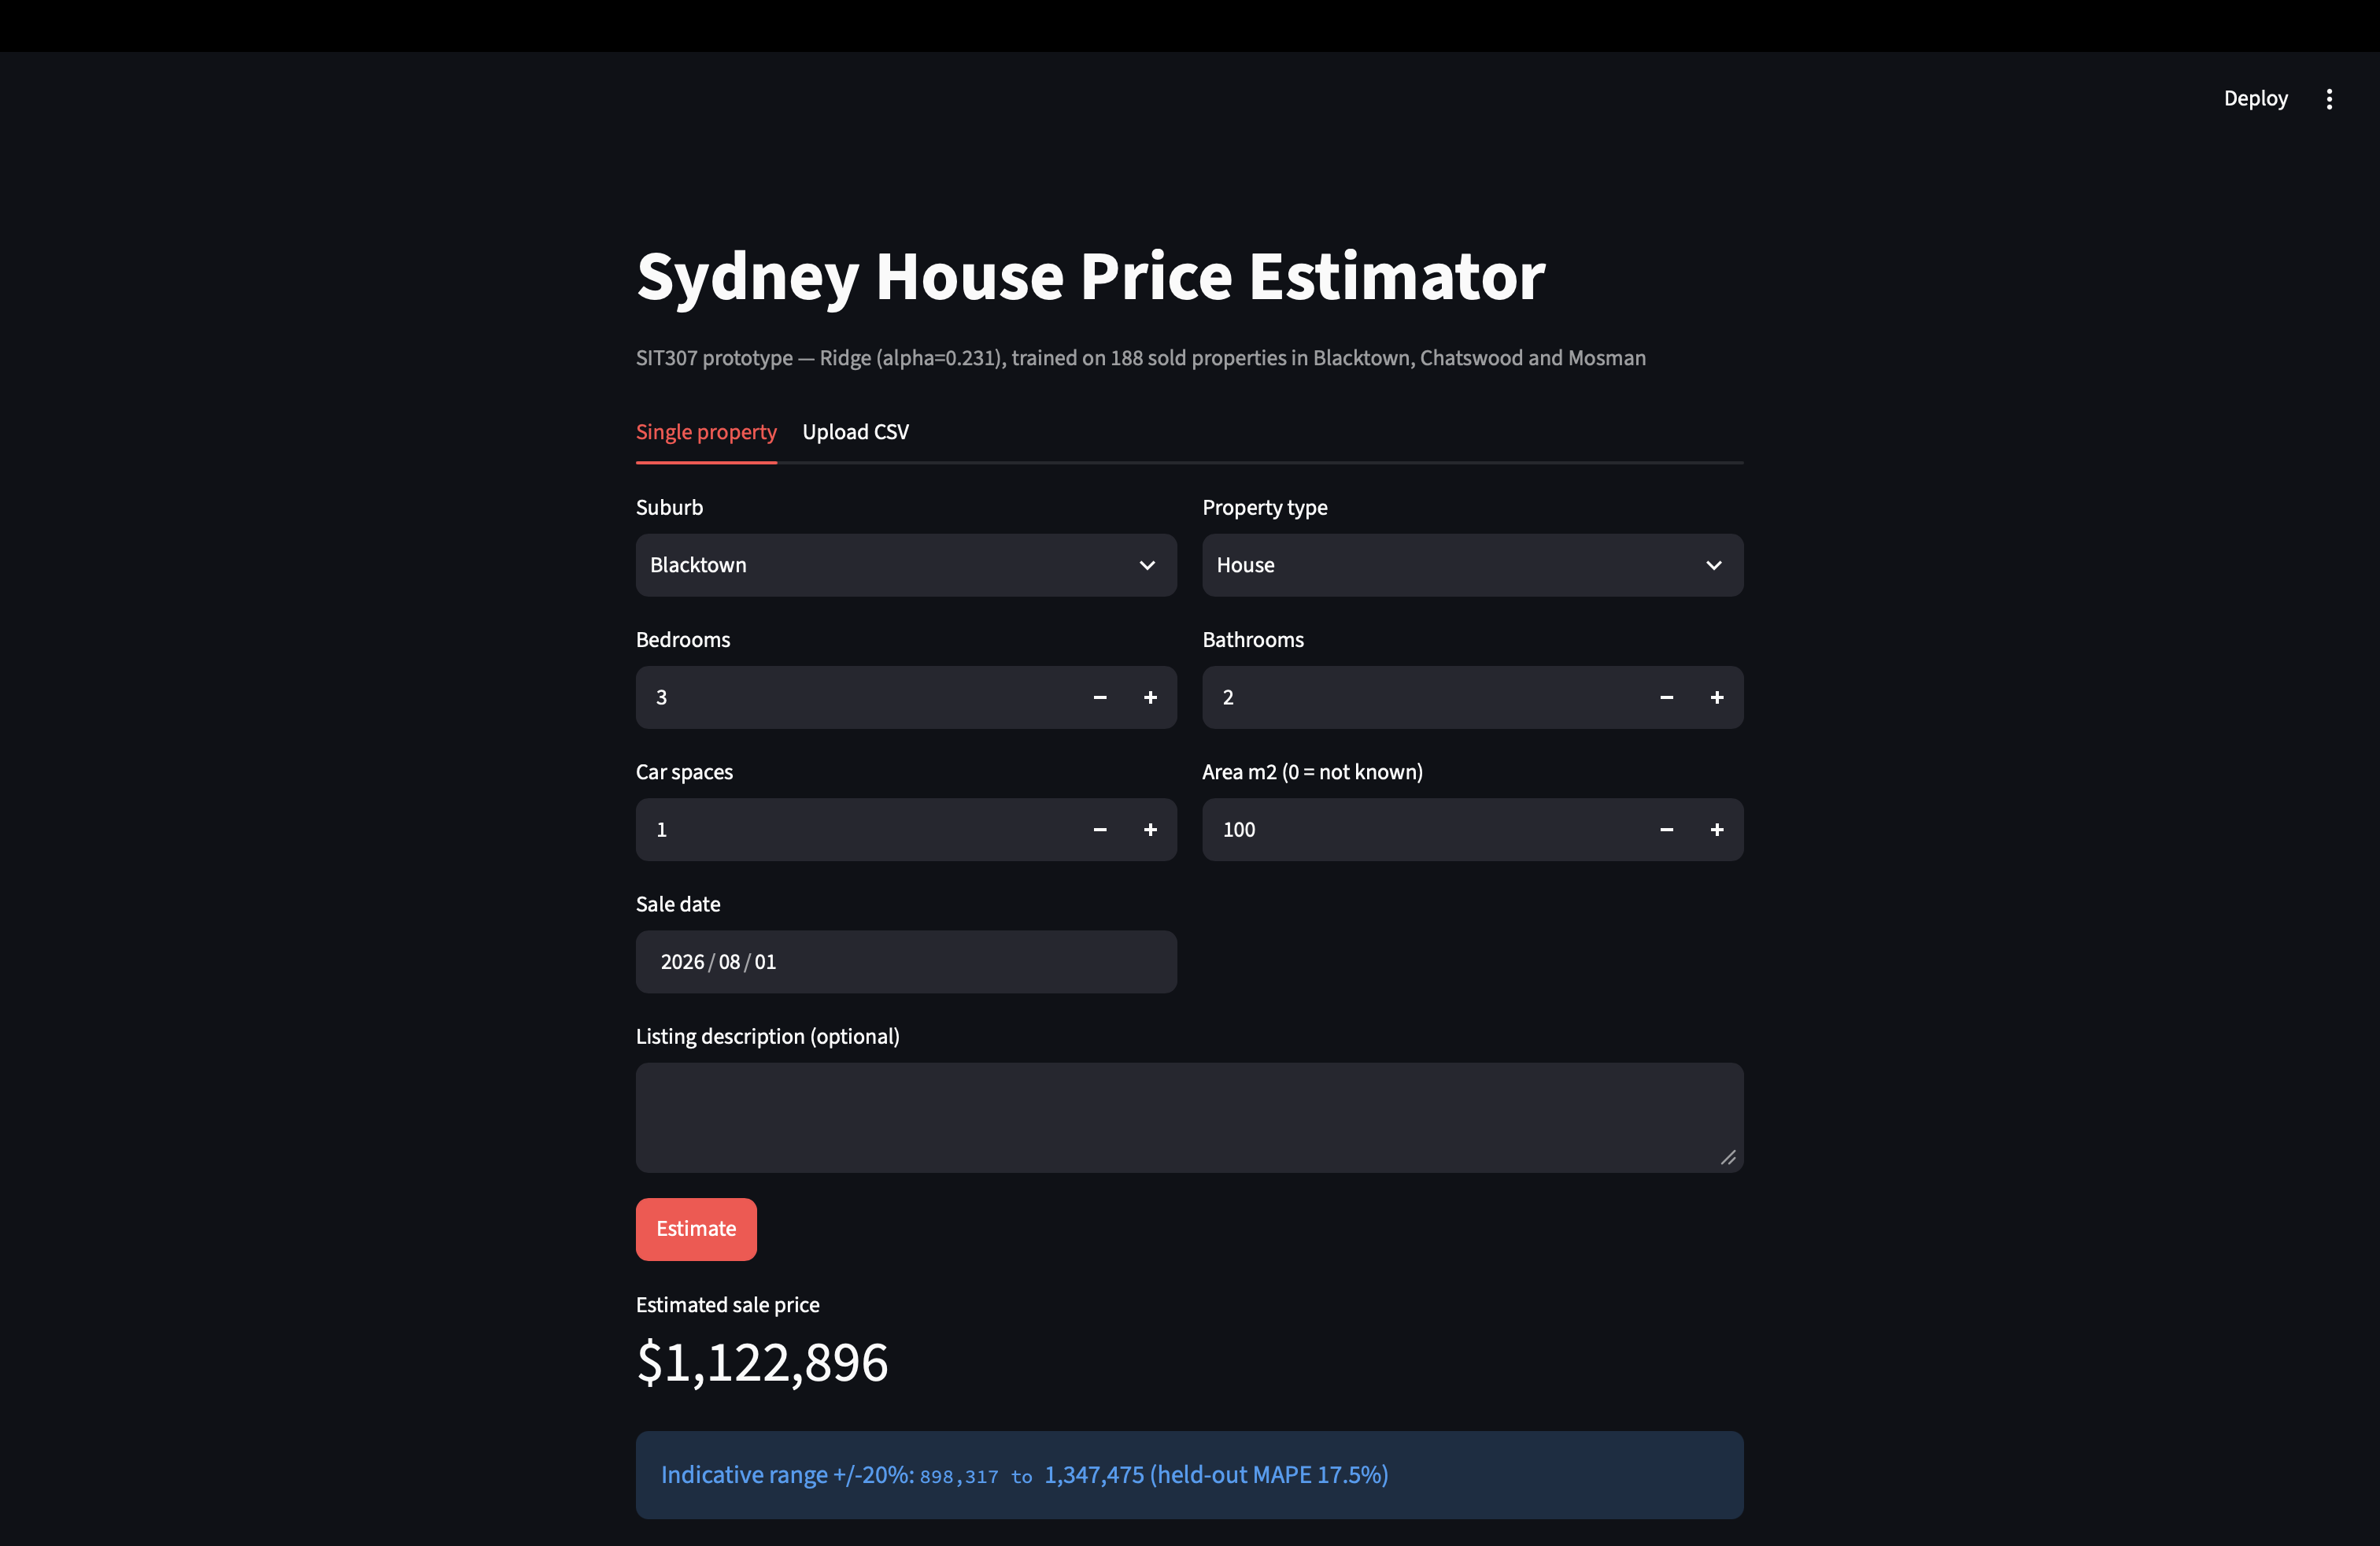
\includegraphics[width=\linewidth]{figures/p5_app_single.png}
\caption{Single-property estimate.}\end{subfigure}\hfill
\begin{subfigure}{0.49\textwidth}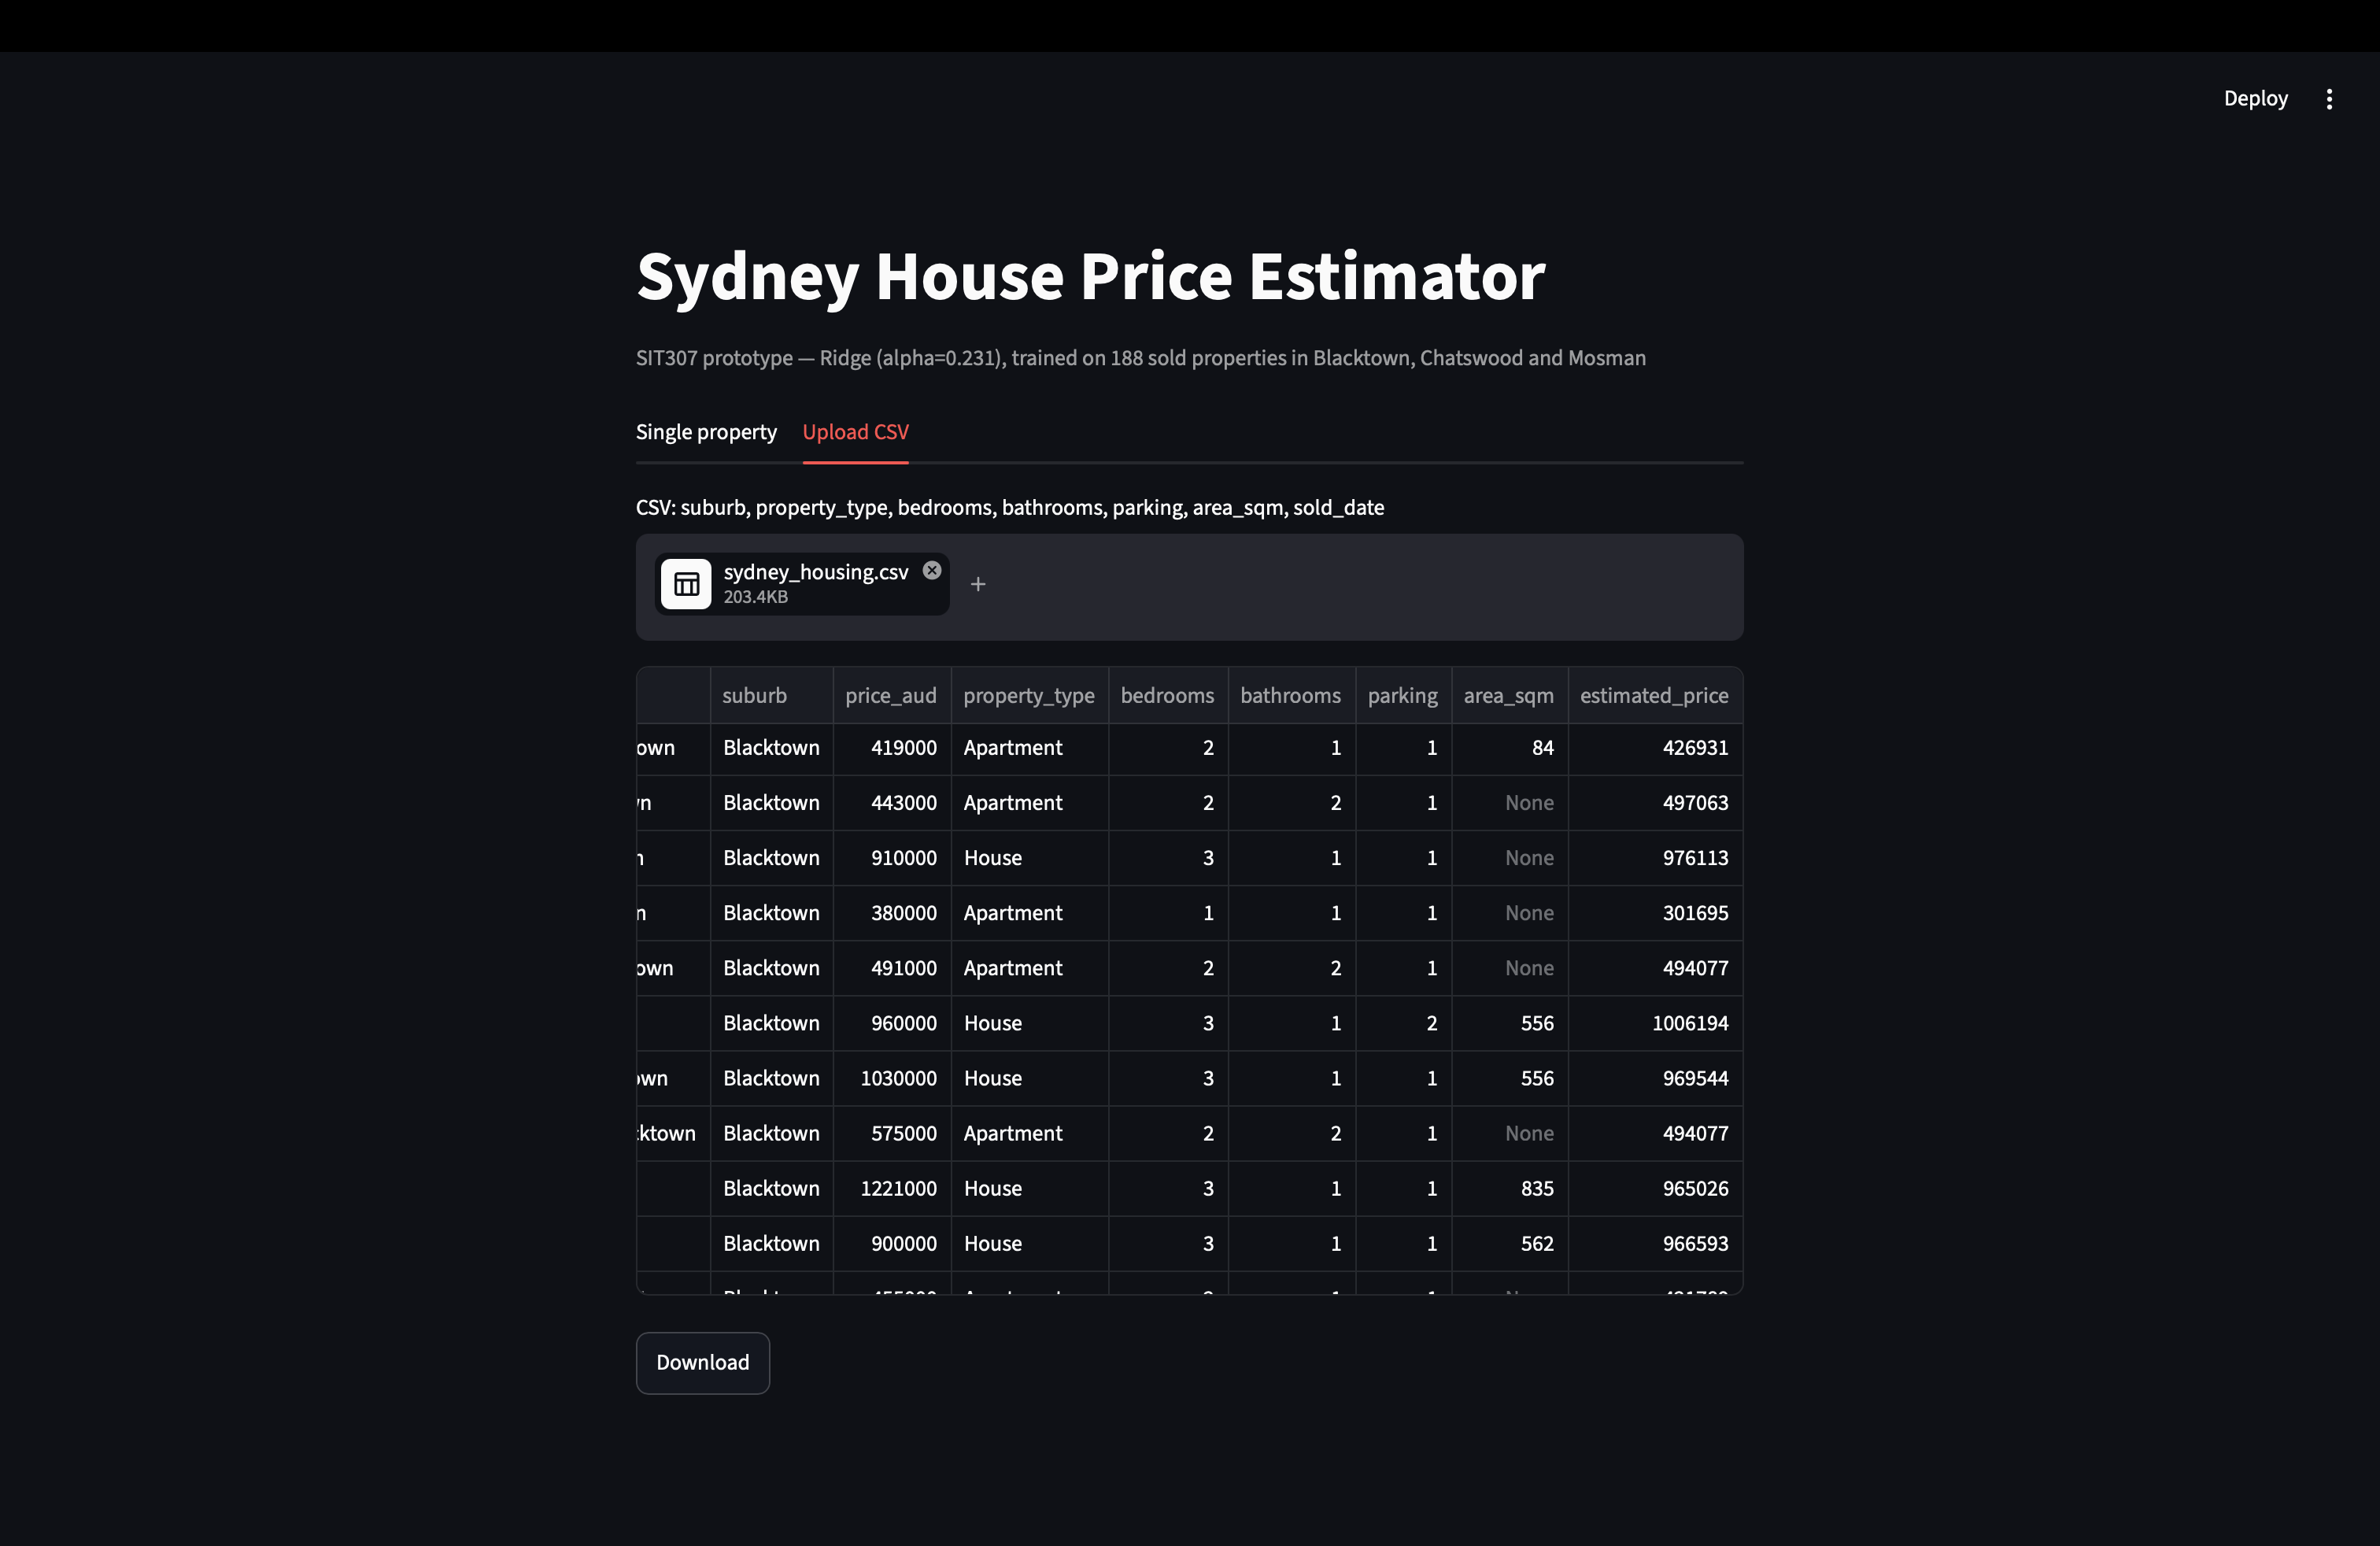
\includegraphics[width=\linewidth]{figures/p5_app_csv.png}
\caption{Batch estimates from an uploaded CSV.}\end{subfigure}
\caption{The Streamlit application. Estimates are shown with a $\pm 20\%$ band, and
warnings fire on the cases Section~4 identified as unreliable.}
\label{fig:app}
\end{figure}


\subsection{Reflection}

\textbf{Data collection was the real bottleneck, not modelling.} Only 188 of the 239
listings passed the completeness rule, and almost every later limitation comes back to
that number. The learning curves were still improving at the end, so more sales would
have helped more than a better estimator. Choosing which rows to drop also turned out to
be a modelling decision. Exempting \texttt{area\_sqm} kept the suburbs balanced, but
it meant imputing that column for a third of the sample.

\textbf{Evaluation choices changed the conclusions.} When we scored in-sample instead of
out-of-fold, the top two models swapped places. Likewise, MAPE computed on the logged
target read 1.17\% rather than the actual 16.8\%.

\textbf{Accuracy versus deployability.} Noticeably, the most useful signals were also the
hardest to serve. Since \texttt{area\_sqm} is a third missing, the application has to
accept a blank and fall back on the training median, while the \texttt{kw\_*} flags
added almost nothing. Therefore, the deployed model only asks for fields that can be read
off a listing in seconds, and we accept about $\pm 20\%$ error in exchange for an
interface that needs no preparation.

\textbf{Bias and fairness.} Three suburbs do not represent Sydney, and even within them
coverage is uneven, with 79 Blacktown sales against 47 in Mosman. The error follows the
same pattern, at 11.7\% against 20.9\%. Moreover, suburb is an explicit input and SEIFA
turned out to be the suburb label restated, so the model encodes existing spatial
inequality and would carry it into any decision it informs.

\textbf{Given more resources.} First, a longer collection window would separate
seasonality from trend and fill in the sparse Mosman tail. Second, capturing
\texttt{area\_sqm} at collection time would remove the need to impute it. Finally,
nested cross-validation would remove the optimism still left in the CV figures.


%=========================================================


\newpage
\bibliographystyle{ieeetr} % or another style like plain, apa, etc.
\bibliography{literature}
\nocite{*}

\end{document}
